\documentclass{article}
\usepackage{graphicx}
\usepackage[section]{placeins}
\usepackage{listings}
\begin{document}

\title{Practical work 1\protect\\ Distributed System}
\author{Distributed System Group 5\\ Nguyen Trac Thanh - Bi8-170\\ Le Quang Vinh - Bi8-188 \\ Dao Anh Hong - Bi8-068 \\ Dang Minh Duc - Bi8-047 \\ Cao Phuong Linh - Bi7-091} 

\maketitle
\pagenumbering{gobble}
\newpage
\tableofcontents

\pagenumbering{arabic}
\newpage
\section{Architecture}
\subsection{FTP}
\begin{figure}
    \centering
    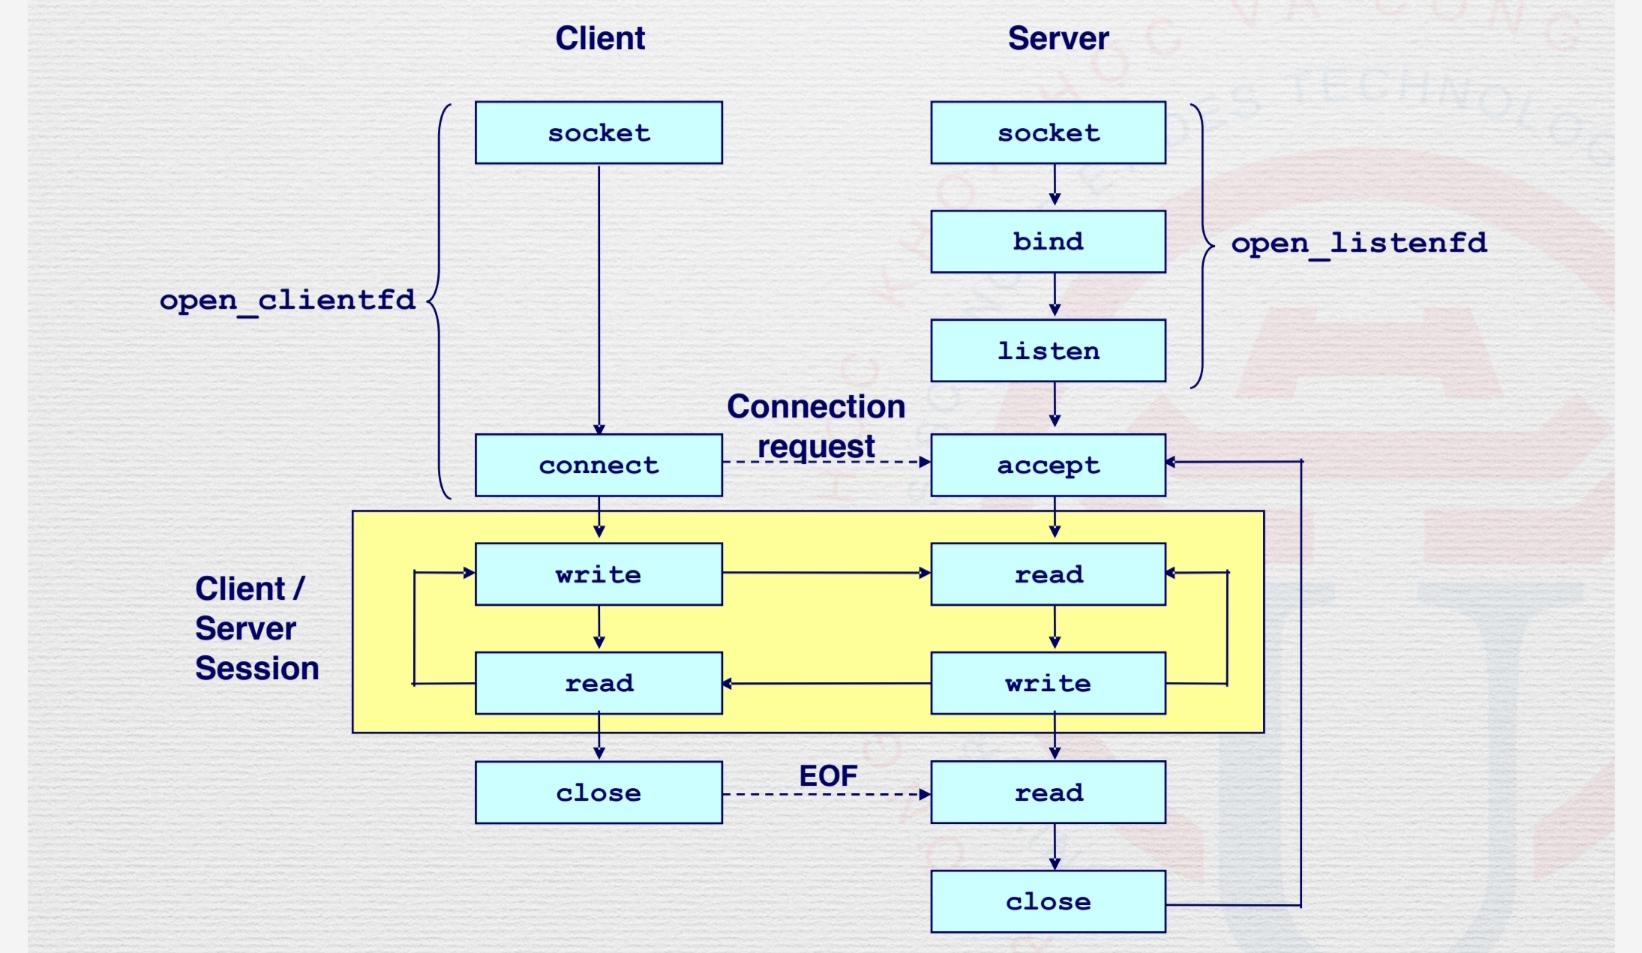
\includegraphics[height=\textheight, width=\textwidth,keepaspectratio]{Protocol.jpg}
    \caption{File transfer protocol}
\end{figure}




\newpage
\section{Code implementation}
\subsection{Server}
\begin{lstlisting}
#include <stdio.h>
#include <stdlib.h>
#include <string.h>
#include <sys/types.h>
#include <sys/socket.h>
#include <netdb.h>

int main() {
int ss, cli, pid;
struct sockaddr_in ad;
char s[100];
socklen_t ad_length = sizeof(ad);

// create the socket
ss = socket(AF_INET, SOCK_STREAM, 0);

// bind the socket to port 12345
memset(&ad, 0, sizeof(ad));
ad.sin_family = AF_INET;
ad.sin_addr.s_addr = INADDR_ANY;
ad.sin_port = htons(12345);
bind(ss, (struct sockaddr *)&ad, ad_length);

// then listen
listen(ss, 0);

while (1) {
// an incoming connection
cli = accept(ss, (struct sockaddr *)&ad, &ad_length);

pid = fork();
if (pid == 0) {
// I'm the son, I'll serve this client
printf("client connected\n");
while (1) {
// it's client turn to chat, I wait and read message from client
read(cli, s, sizeof(s));
printf("client says: %s\n",s);

// now it's my (server) turn
printf("server>", s);
scanf("%s", s);
write(cli, s, strlen(s) + 1);
}
return 0;
}
else {
// I'm the father, continue the loop to accept more clients
continue;
}
}
// disconnect
close(cli);

}

\end{lstlisting}
\subsection{Client}
\begin{lstlisting}

#include <stdio.h>
#include <stdlib.h>
#include <string.h>
#include <sys/types.h>
#include <sys/socket.h>
#include <netdb.h>

int main(int argc, char* argv[]) {
int so;
char s[100];
struct sockaddr_in ad;

socklen_t ad_length = sizeof(ad);
struct hostent *hep;

// create socket
int serv = socket(AF_INET, SOCK_STREAM, 0);

// init address
hep = gethostbyname(argv[1]);
memset(&ad, 0, sizeof(ad));
ad.sin_family = AF_INET;
ad.sin_addr = *(struct in_addr *)hep->h_addr_list[0];
ad.sin_port = htons(12345);

// connect to server
connect(serv, (struct sockaddr *)&ad, ad_length);

while (1) {
// after connected, it's client turn to chat

// send some data to server
printf("client>");
scanf("%s", s);
write(serv, s, strlen(s) + 1);

// then it's server turn
read(serv, s, sizeof(s));

printf("server says: %s\n", s);
}
}


\end{lstlisting}


\newpage
\section{Who did what?}

  Nguyen Trac Thanh and Le Quang Vinh : Rewrite the code from Dr.Son source code and execute it.
 \\
 \\
 Dang Minh Duc and Cao Phuong Linh : Design and write the report.
 \\ 
 \\
 Dao Anh Hong: Research about the protocol.
\end{document}
\end{center}



\end{document}
